

\begin{frame}{Introducción a la XAI}
    \dificultyLevel{1}
    \begin{itemize}[<+- | alert@+>]
        \item La capacidad de los modelos de IA ha crecido exponencialmente.
        \item Esto aumenta su complejidad y dificulta su comprensión.
        \item La \textbf{XAI} (Explainable Artificial Intelligence) busca explicar decisiones y predicciones de los modelos.
        \begin{figure}[htbp]
        	\centering
        	\begin{subfigure}[b]{0.45\textwidth}
        		\centering
        		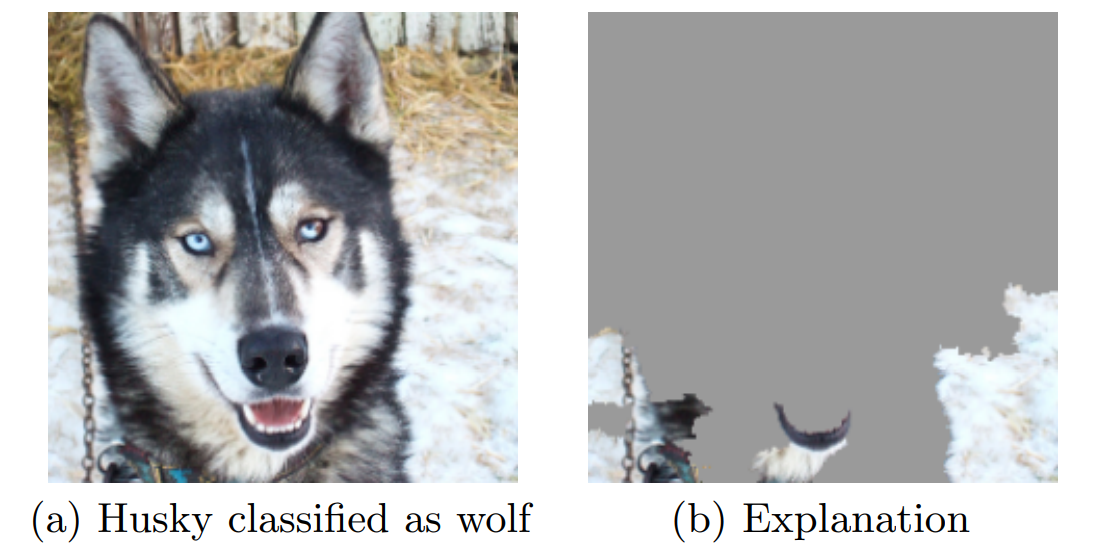
\includegraphics[width=\textwidth]{pic/img/XAI/explainabilityExample.png}
        	\end{subfigure}
        	\hfill
        	\begin{subfigure}[b]{0.45\textwidth}
        		\centering
        		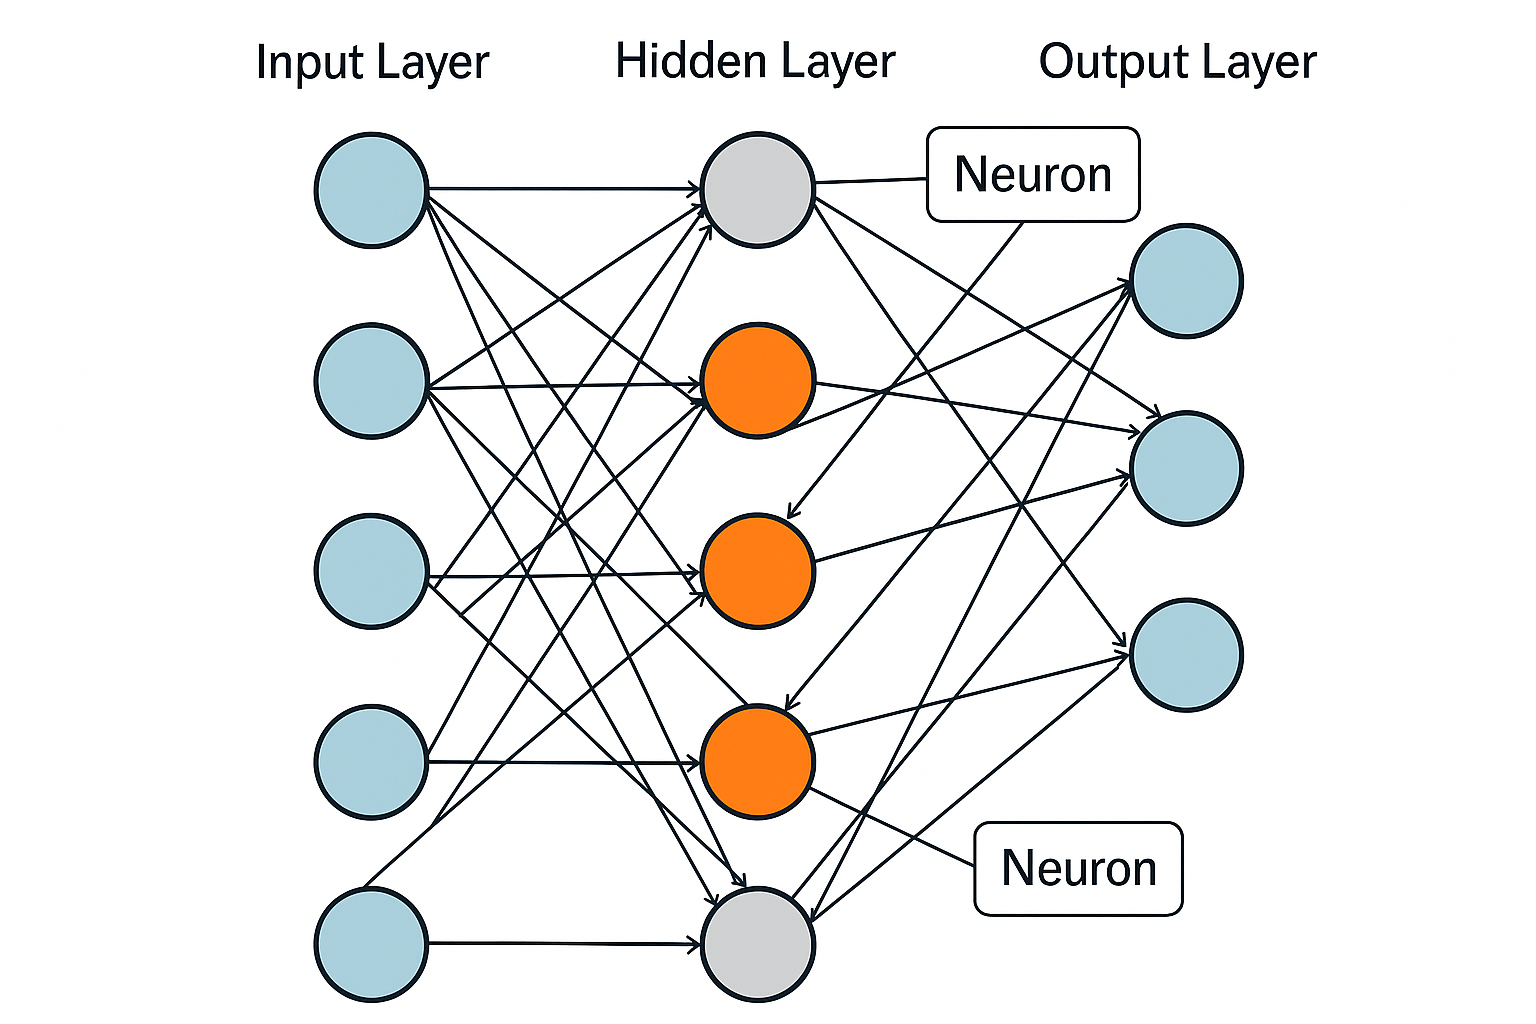
\includegraphics[width=\textwidth]{pic/img/XAI/interpretabilityExample.png}
        	\end{subfigure}
        	
        \end{figure}
    \end{itemize}
    
    \only<1>{
    	\vspace{-140px}
    	\begin{figure}
    		\centering
    		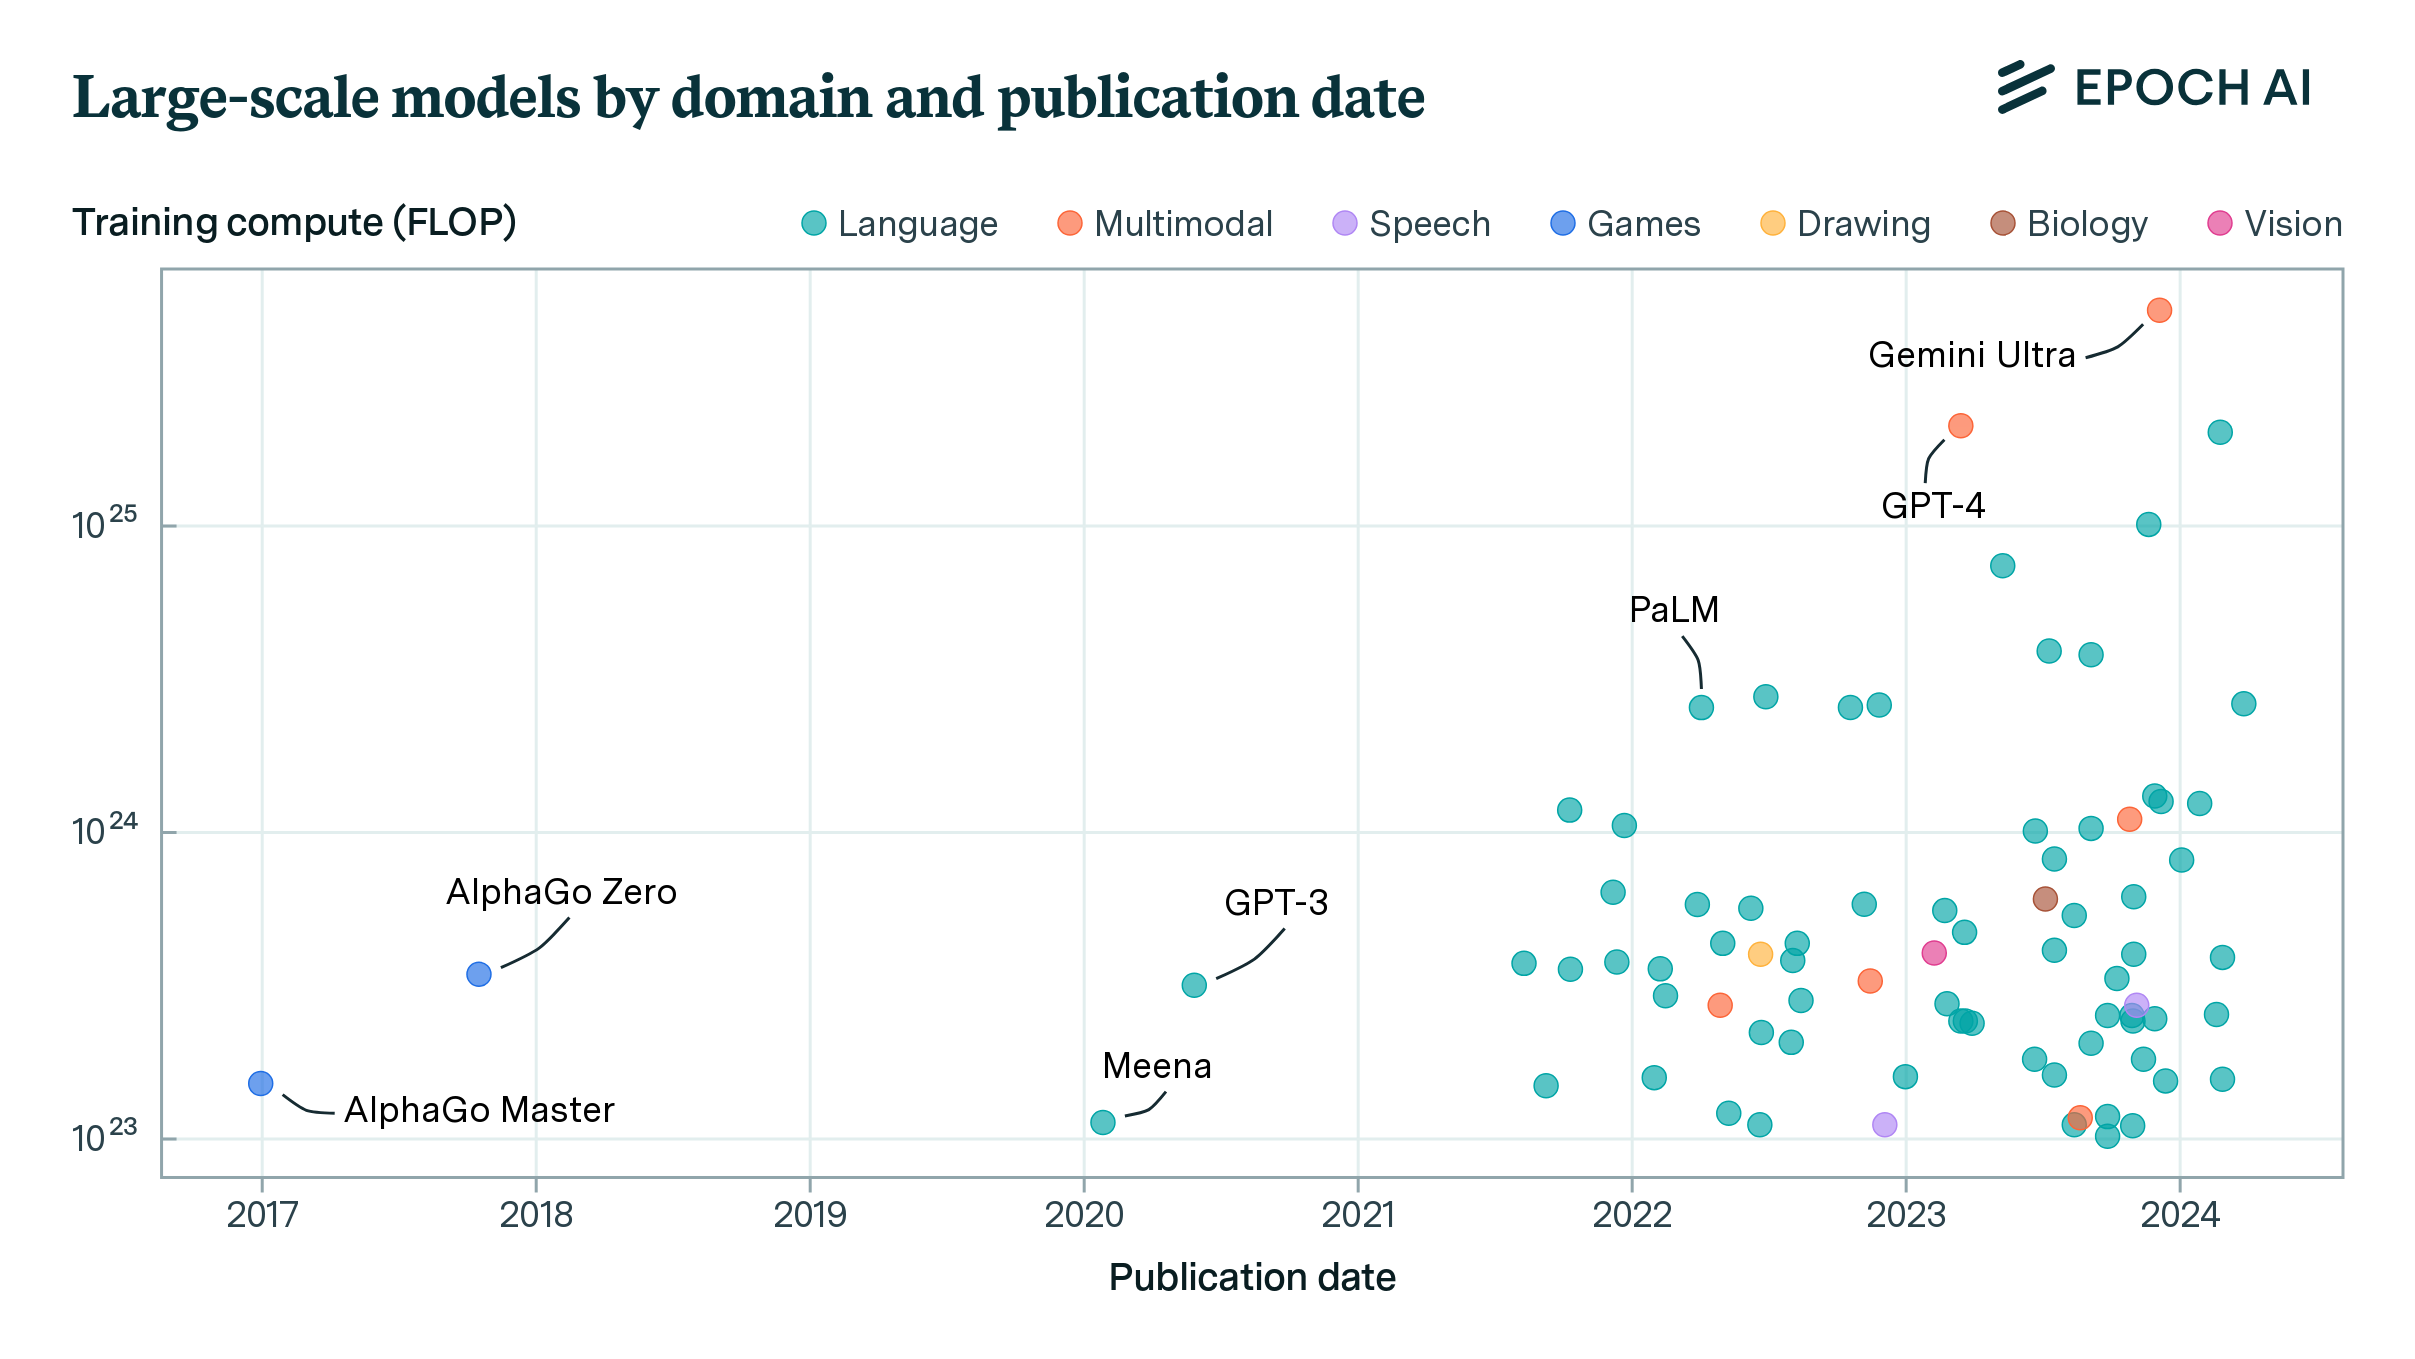
\includegraphics[width=\textwidth]{pic/img/XAI/large-scale-models-by-domain-and-date.png}
    \end{figure}}
\end{frame}

\begin{frame}{Before and after XAI}
        \begin{figure}
		\centering
		\begin{subfigure}[b]{0.45\textwidth}
			\centering
			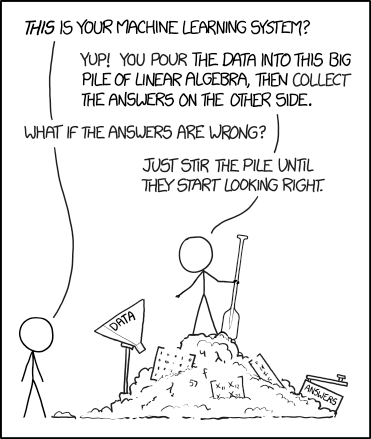
\includegraphics[width=\textwidth]{pic/img/XAI/XAIMeme.png}
		\end{subfigure}
		\hfill
		\pause 
		\begin{subfigure}[b]{0.45\textwidth}
			\centering
			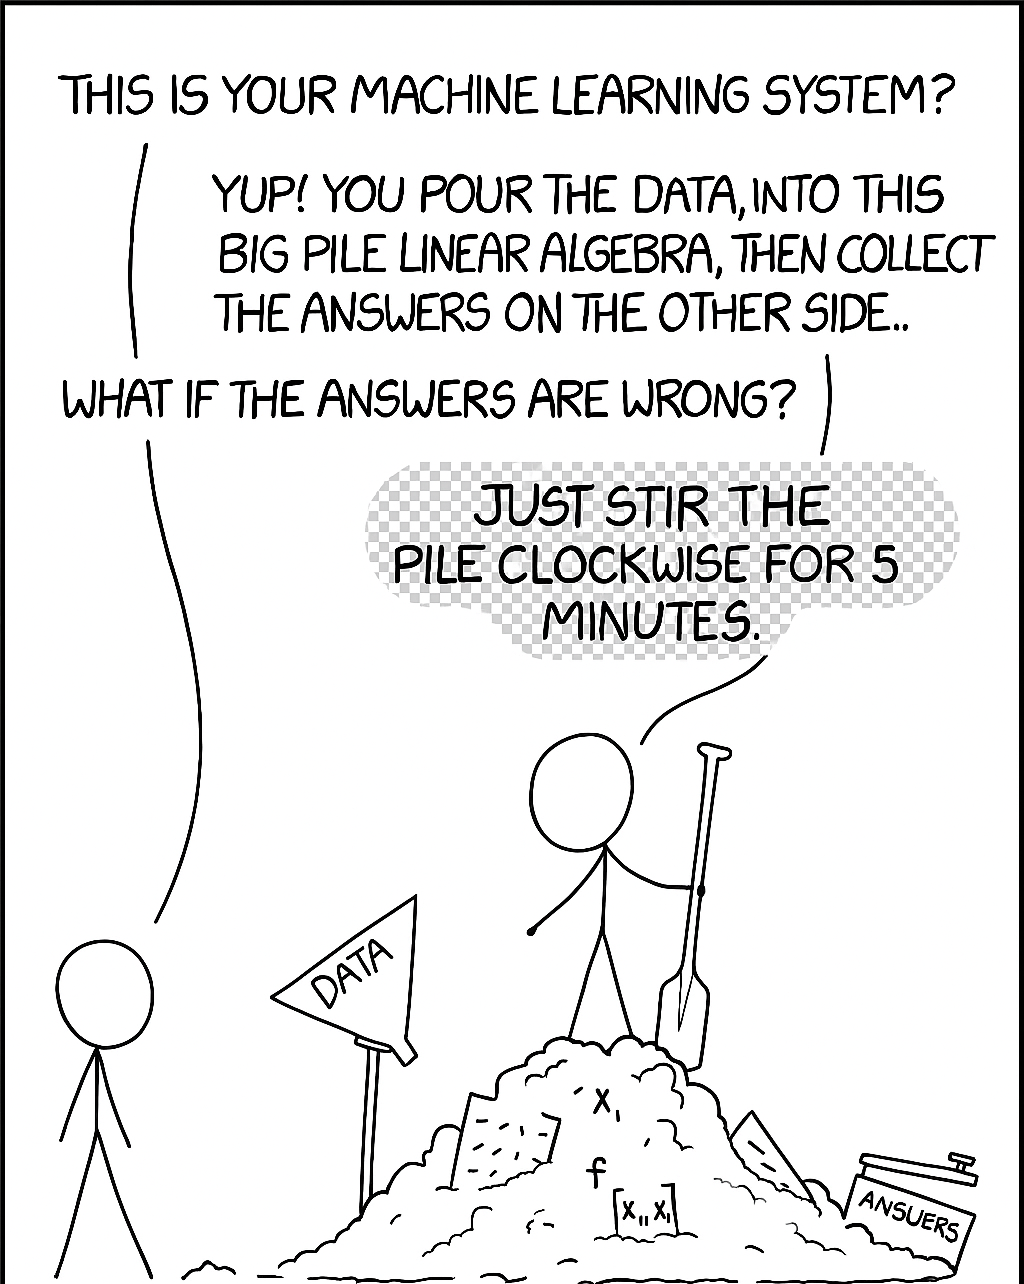
\includegraphics[width=\textwidth]{pic/img/XAI/XAIMemeAfter.png}
		\end{subfigure}
\end{figure}
\end{frame}

\begin{comment}
	\item Dos grandes ramas:
	\begin{itemize}
		\item \textbf{Explicabilidad}: Explicaciones externas de las decisiones.
		\item \textbf{Interpretabilidad}: Comprensión de la representación interna.
	\end{itemize}
	\item En esta tesis nos vamos a enfocar en un método de la rama de la explicabilidad.
\end{comment}

\begin{frame}{Tipos de métodos en XAI}
    \dificultyLevel{1}

	\begin{figure}[htbp]
		\centering
		\begin{subfigure}[b]{0.40\textwidth}
			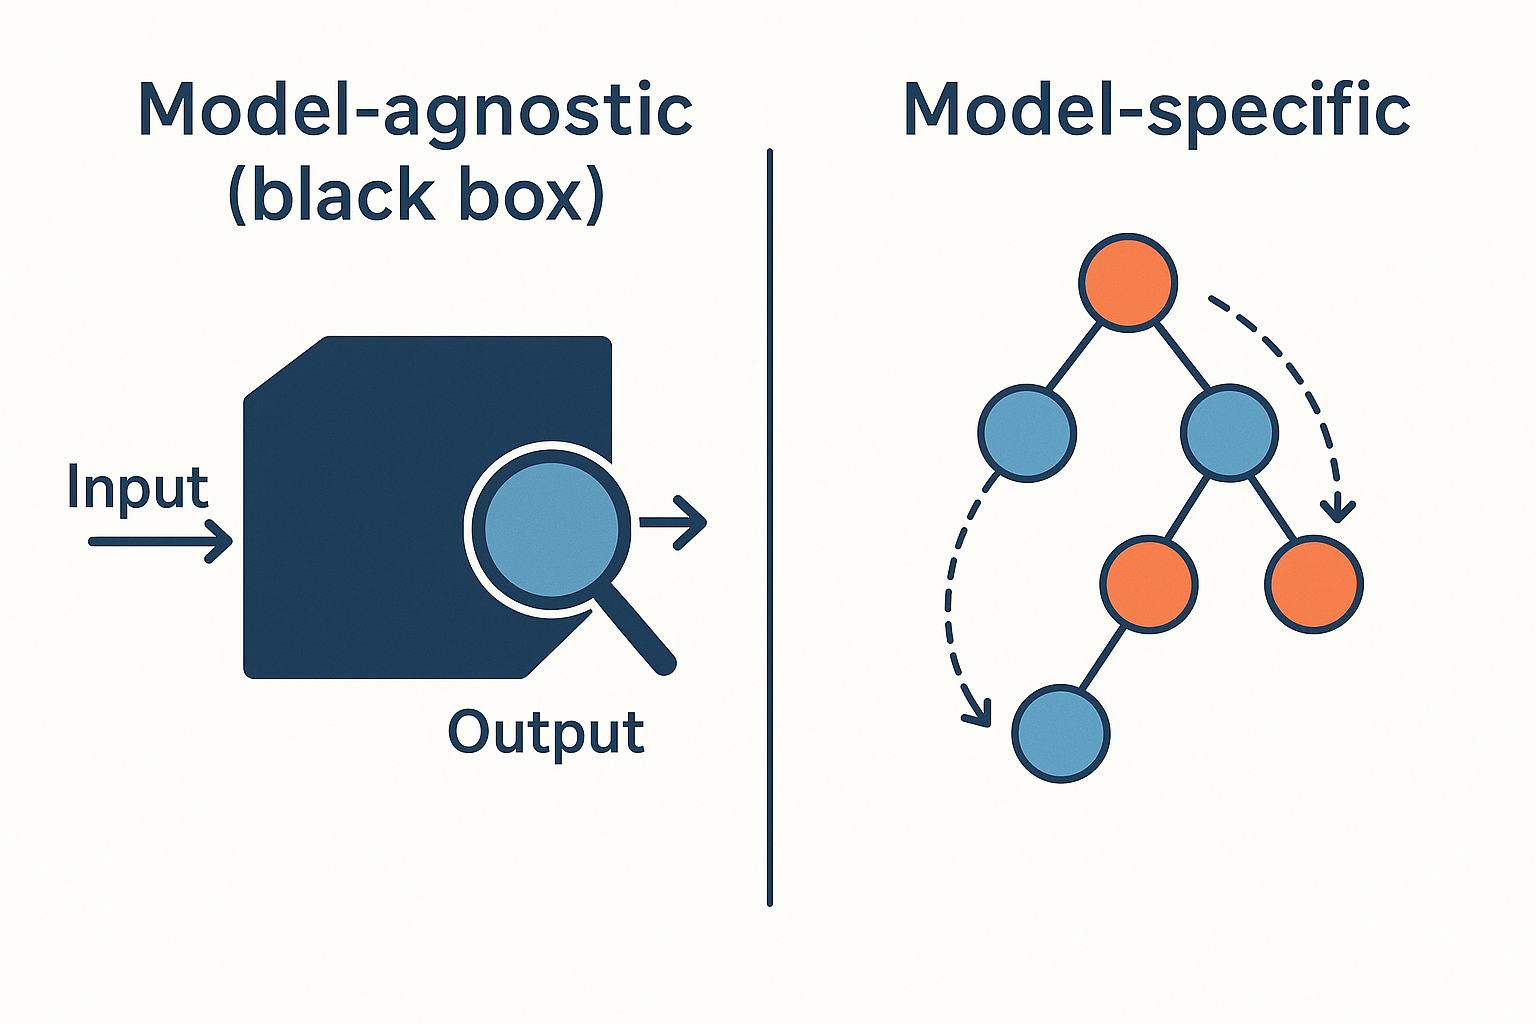
\includegraphics[width=\textwidth]{pic/img/XAI/modelSpecificvsAgnostic.png}
		\end{subfigure}
		 \pause
		\hfill
		\begin{subfigure}[b]{0.40\textwidth}
			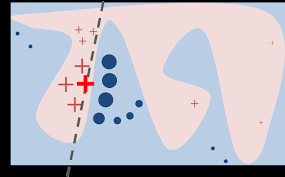
\includegraphics[width=\textwidth]{pic/img/XAI/localVsGlobalPrediction.png}
		\end{subfigure}
		\pause
		\hfill
		\begin{subfigure}[b]{0.40\textwidth}
			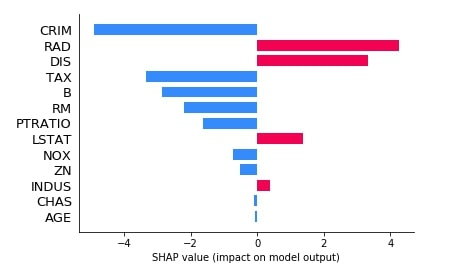
\includegraphics[width=\textwidth]{pic/img/XAI/featureRelevanceExample.jpg}
		\end{subfigure}
	\end{figure}
	
    \pause
    \textit{No existe una definición universal de ``explicación''. Las técnicas actuales son aproximaciones pragmáticas.}
\end{frame}

\begin{frame}{SHAP: Un método de feature attribution}
    \dificultyLevel{1}
    \begin{itemize}[<+- | alert@+>]
        \item SHAP se basa en los valores de Shapley de teoría de juegos, los cuáles veremos más adelante.
        \item Características:
        \begin{itemize}
            \item Agnóstico al modelo.
            \item Alcance local (aunque puede ser global)
            \item Feature attribution.
        \end{itemize}
        %\item SHAP es un framework de explicabilidad que incluye métodos agnósticos y específicos al modelo.
        %\item Problema: Calcularlo es costoso (\NPcomplete{} en casos simples).
    \end{itemize}
\end{frame}

\begin{frame}{ASV vs SHAP: Incorporando Causalidad}
    \dificultyLevel{2}
    \begin{itemize}[<+- | alert@+>]
        \item \textbf{ASV (Asymmetric Shapley Values)} incorpora la estructura causal de los datos al calcular la relevancia de los features.
        \item Veamos un ejemplo de cómo ASV incorpora esta información.
        \begin{itemize}
            \item Modelo: Red neuronal que predice si el sueldo anual de una persona es mayor o menor a 50.000 dolares.
            \item Datos de entrenamiento: \textit{Census Income} dataset del UC Irvine. 
            \item Métricas a evaluar: ASV y SHAP globales. %(on/off manifold) globales. %El cálculo global se realiza a través del promedio de las explicaciones locales para cada instancia.

            %Para este experimento se calculan dos variaciones de SHAP, una \emph{off-manifold} y otra \emph{on-manifold}, la diferencia es la función de probabilidad que ambas usan. En el enfoque \emph{on-manifold} se respetan las restricciones que hay entre las distintas variables, por ejemplo a la hora de calcular SHAP se va a descartar cualquier instancia tal que $age=3 \land occupation = teacher$, ya que eso no es posible. Pero en el enfoque \emph{off-manifold} no va a haber ninguna restricción a la hora de combinar los distintos valores de cada feature. Estas restricciones se obtienen a través de las correlaciones entre las distintas variables del dataset.
        \end{itemize}
        
    \end{itemize}
\end{frame}

\begin{frame}{Digrafo causal del Census Income Dataset}
    \dificultyLevel{1}
    \begin{figure}[h!]
        \centering
        \begin{tikzpicture}[
            scale=0.4, transform shape, % Escalado general
            node distance=1cm and 2.8cm,
            every node/.style={draw, rounded corners, font=\scriptsize, minimum width=1.6cm, minimum height=0.6cm, align=center},
            arrow/.style={-{Latex}, very thin, opacity=0.4}
        ]
        
        % Ancestors (A)
        \node (age)                    {age};
        \node[below=of age] (sex)      {sex};
        \node[below=of sex] (native)   {native country};
        \node[below=of native] (race)  {race};
        
        % Descendants (D)
        \node[right=of age]     (marital)    {marital-status};
        \node[below=of marital] (education)  {education};
        \node[below=of education] (relation) {relationship};
        \node[below=of relation] (occupation){occupation};
        \node[below=of occupation] (capgain) {capital-gain};
        \node[below=of capgain] (hours)      {hours-per-week};
        \node[below=of hours]   (caploss)    {capital-loss};
        \node[below=of caploss] (workclass)  {workclass};
        
        % Aristas: de cada A a cada D
        \foreach \a in {age, sex, native, race} {
            \foreach \d in {marital, education, relation, occupation, capgain, hours, caploss, workclass} {
                \draw[arrow] (\a) -- (\d);
            }
        }
        
        \end{tikzpicture}
        \caption*{Dígrafo causal: aristas de $A = \{age, sex, native\ country, race\}$ hacia $D = \set{marital, education, relation, occupation, capital-gain, hours, capital-loss, workclass}$}
    \end{figure}

\end{frame}

\begin{frame}{Resultados ASV vs SHAP}
    \dificultyLevel{1}
    \begin{figure}
        \centering
        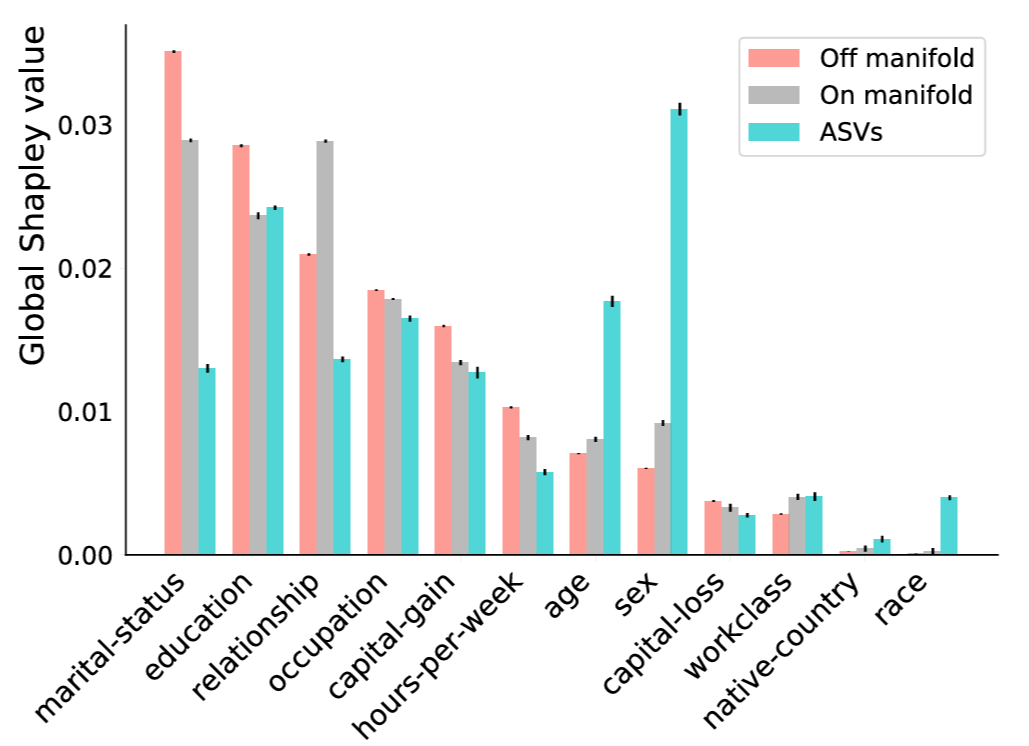
\includegraphics[width=0.7\linewidth]{pic/img/asvPaperPlotExample.png}
        \caption*{Comparación de los valores globales de SHAP y ASV para el Census Income Dataset.}
    \end{figure}
    %Ellos para calcular ASV y SHAP dicen que usan "are similarly Monte Carlo estimates with 106 samples." Entendemos que samplearon los toposorts (en este caso es fácil pues solo que tienen hacer una permutación de A + una permutación de D) y luego evaluaron las predicciones promedio. 
    %Podemos ver que ASV detecta relaciones entre los datos que SHAP no.
\end{frame}

\begin{frame}{Objetivo de la tesis}
    \dificultyLevel{1}
    \begin{itemize}[<+- | alert@+>]
        \item Problema de ASV: Es costoso calcularlo, pero a diferencia de SHAP, para algunos modelos que SHAP es difícil, ASV es tratable. 
        \item Objetivo inicial de la tesis: Calcular ASV en \emph{tiempo polinomial} para una familia de \textit{digrafos causales} %y para una \textit{distribución}.
        \item Todos los algoritmos mencionados los pueden encontrar en:
        \begin{table}
        \centering
        \begin{tabular}{ll}
            \toprule
            \textbf{Repo} & \url{https://github.com/EchuCompa/pasantia-BICC} \\
            \bottomrule
        \end{tabular}
        \end{table}
    \end{itemize}
\end{frame}
